\documentclass[xcolor=dvipsnames]{beamer}
%\documentclass[handout,xcolor=dvipsnames]{beamer}

% == Packages for beamer
\usepackage{xcolor}
\usepackage{graphicx}
\usepackage{fancybox}
\usepackage{hyperref}
\usepackage{amsmath,amssymb,amsfonts,bm}
\usepackage{wasysym}
\usepackage{colortbl}
\usepackage{booktabs}
\usepackage[english]{babel}
\usepackage{times}
\usepackage[T1]{fontenc}

% == Other Packages
\usepackage{rotating}
\usepackage{latexsym}
\usepackage{ulem}
\usepackage{appendixnumberbeamer}

% == theme & colors
\usetheme{Warsaw}
\usepackage{helvet}
\definecolor{someblue}{rgb}{0,.1,0.8}
\definecolor{dgreen}{rgb}{0,.6,0.8}
\useoutertheme{infolines}

% == New Commands
\newcommand\spacingset[1]{\renewcommand{\baselinestretch}{#1}\small\normalsize}
\renewcommand\r{\right}
\renewcommand\l{\left}
\newcommand\makegaps{\addtolength{\itemsep}{.25\baselineskip}}
\newcommand\makebiggaps{\addtolength{\itemsep}{.5\baselineskip}}

% = For stats & econometrics
\renewcommand{\epsilon}{\varepsilon}
\newcommand\ud{\mathrm{d}}
\newcommand\dist{\buildrel\rm d\over\sim}
\newcommand\ind{\stackrel{\rm indep.}{\sim}}
\newcommand\iid{\stackrel{\rm i.i.d.}{\sim}}
\newcommand\logit{{\rm logit}}
\newcommand\cA{\mathcal{A}}
\newcommand\cN{\mathcal{N}}
\newcommand\E{\mathbb{E}}
\newcommand\V{\mathbb{V}}
\newcommand\cJ{\mathcal{J}}
\newcommand\y{{\bm y}}
\newcommand\Y{{\bm Y}}
\newcommand\X{{\bm X}}
\newcommand\x{{\bm x}}
\newcommand\eps{{\bm\varepsilon}}
\newcommand\zero{{\bm 0}}
\newcommand\be{{\bm\beta}}
\renewcommand\b{{\bm b}}
\newcommand\C{{\bm C}}
\newcommand\D{{\bm D}}
\newcommand\I{{\bm I}}
\newcommand\Z{{\bm Z}}
\newcommand\eeta{{\bm \eta}}
\newcommand{\Var}{\mathrm{Var}}
\newcommand{\Cov}{\mathrm{Cov}}

\DeclareMathOperator*\plim{plim}
\DeclareMathOperator\rank{rank}
\newcommand\indep{\protect\mathpalette{\protect\independenT}{\perp}}
\DeclareMathOperator{\sgn}{sgn}
\def\independenT#1#2{\mathrel{\rlap{$#1#2$}\mkern2mu{#1#2}}}

\newtheorem{assumption}{Assumption}
\newtheorem{iass}{Identification Assumption}
\newtheorem{ires}{Identfication Result}
\newtheorem{estm}{Estimand}
\newtheorem{esti}{Estimator}

\newcommand{\notindep}{{\bot\negthickspace\negthickspace\bot}{\negthinspace
  \negmedspace \negthickspace \negthickspace \diagup
  \;}}
\newcommand{\bs}{\boldsymbol}
\newcommand{\mb}{\mathbf}
\newcommand{\real}{\mathbb{R}}
\renewcommand{\u}{\ensuremath{\mb{u}}}
\renewcommand{\v}{\ensuremath{\mb{v}}}
\newcommand{\U}{\ensuremath{\mb{U}}}
\newcommand{\M}{\ensuremath{\mb{M}}}
\renewcommand{\b}{\ensuremath{\bs{\beta}}}
\newcommand{\e}{\ensuremath{\bs{\epsilon}}}
\newcommand{\bhat}{\ensuremath{\hat{\bs{\beta}}}}
\newcommand{\XX}{\ensuremath{\X'\X}}
\newcommand{\XXinv}{\ensuremath{\left(\XX\right)^{-1}}}
\newcommand{\hatsig}{\ensuremath{\hat{\sigma}^2}}
\newcommand{\sig}{\ensuremath{\sigma^2}}
\newcommand{\hatmat}{\ensuremath{\X \XXinv \X'}}
\newcommand{\ehat}{\ensuremath{\hat{\e}}}
\newcommand{\tr}{\text{tr}}
\newcommand{\Sig}{\ensuremath{\bs{\Sigma}}}
\newcommand{\SigInv}{\ensuremath{\bs{\Sigma^{-1}}}}
\newcommand{\W}{\ensuremath{\mb{W}}}

\graphicspath{{figures/}{images/}}

\title[]{Experiments: Part II}
\subtitle[ ]{PS200C Quant Methods in Politics, Spring 2026}
\author[Hazlett]{Chad Hazlett }
\institute[UCLA]{UCLA\\[1ex]
  \texttt{chazlett@ucla.edu}
}
\date{}

\begin{document}

\begin{frame}
  \titlepage
\end{frame}

\begin{frame}{Where we are}
\begin{itemize}
\item Part I: random assignment makes the simple difference in means an
  unbiased estimator of the ATE. \medskip
\item Part II: \textbf{unbiased is not enough.} The same experiment can be
  run well or badly. Today is about what ``well'' means and how design
  and analysis together deliver it.\medskip
\item Roadmap:
\begin{enumerate}
\footnotesize
\item Why unbiasedness isn't the whole story (and balance as a hook)
\item Covariate adjustment (precision, not bias)
\item Blocking (better-than-random balance by design)
\item Non-independence: dependent residuals and clustered assignment
\item Wrap and takeaways
\end{enumerate}
\end{itemize}
\end{frame}


% =====================================================================
\section{Design Matters: Unbiased Is Not Enough}
% =====================================================================

\begin{frame}{Diff-in-means is unbiased. So why do anything else?}
\begin{itemize}
\item<1-> Under random assignment, $\hat\tau_{DIM} = \bar Y_{T} - \bar Y_{C}$
  is unbiased for the ATE. We proved this last time. \medskip
\item<2-> But ``unbiased'' is a statement about \textit{averages over
  hypothetical repetitions}. In any \textit{single} experiment, $\hat\tau$
  can land far from $\tau$. \medskip
\item<3-> What we actually care about is something like \textbf{root mean
  squared error}:
  \[
  \mathrm{RMSE}(\hat\tau) = \sqrt{\E[(\hat\tau - \tau)^2]}
  = \sqrt{\Var(\hat\tau) + \mathrm{Bias}(\hat\tau)^2}
  \]
\item<4-> For an unbiased estimator, RMSE = SD. \textbf{Reducing variance is
  the entire game.}
\end{itemize}
\end{frame}


\begin{frame}{Two different ``variances''}
\small
It is easy to conflate two distinct things, both called ``variance.''
\begin{itemize}
\item<1-> \textbf{Actual sampling variance.} $\Var(\hat\tau)$ across
  hypothetical repetitions of the experiment. This is the width of the
  histograms we will draw today. We want this to be small --- it's how
  good our estimator is.
\item<2-> \textbf{Estimated variance / standard error.} A number we
  compute from our \textit{one} dataset, hoping it accurately reflects
  the actual sampling variance. We need this to be roughly correct so
  that confidence intervals cover at the right rate.
\end{itemize}
\medskip
\onslide<3->
\begin{itemize}
\item These can be very different things. A bad SE estimator can produce
  tight intervals around a noisy estimate (under-coverage), or vice versa.
\item Today: \textbf{HC2 (heteroskedasticity-robust)} SEs from \texttt{lm}
  via the \texttt{sandwich} package are the practical default for
  randomized experiments. We'll see they work well for individual
  assignment --- and badly for clustered assignment.
\end{itemize}
\end{frame}


\begin{frame}{Running example: a GOTV experiment}
\small
\begin{itemize}
\item \textbf{Unit:} a registered voter.
\item \textbf{Treatment $D$:} a get-out-the-vote contact (mailer, canvass,
  etc.) vs.\ no contact.
\item \textbf{Outcome $Y$:} did they vote? (0/1)
\item \textbf{Covariates $X$:}
  \begin{itemize}
  \footnotesize
  \item \texttt{past\_turnout}: an index of voting in the last several
    elections. Strong predictor of $Y$. (This is a pre-treatment proxy
    for $Y(0)$.)
  \item \texttt{age}, \texttt{partisan strength}: weaker predictors.
  \end{itemize}
\item \textbf{Structure:} voters are nested in households (4 per household)
  and households in precincts (10 per precinct). 100 precincts, $N=4000$.
\item \textbf{True effect:} $\tau = +0.05$ on the probability of voting.
\item \textbf{We will estimate $\hat\tau$ many times under different designs
  and analyses}, and compare the resulting distributions.
\end{itemize}
\end{frame}


\begin{frame}{What does a single experiment look like? Check balance.}
\small
We randomly assign half the sample to treatment. Then look at the
covariate means by treatment status:

\bigskip
\begin{center}
\begin{tabular}{lrrr}
\toprule
Variable & Treated & Control & Difference \\
\midrule
past\_turnout & -0.028 & -0.001 & -0.027 \\
age & -0.015 & -0.016 & +0.002 \\
partisan & -0.008 & -0.006 & -0.002 \\
\bottomrule
\end{tabular}

\end{center}
\bigskip

\onslide<2->
\begin{itemize}
\item Random assignment guarantees balance \textit{in expectation}, not in
  any one realized sample. Some chance imbalance is inevitable.
\item<3-> Why we ``check balance'' in experiments isn't to detect bias ---
  randomization handles bias. It's to see what kind of \textit{chance
  variation} this realization generated, since that variation is what
  inflates $\Var(\hat\tau)$.
\item<4-> Imbalance on a strong predictor of $Y$ $\Rightarrow$ noisier
  $\hat\tau$. Imbalance on an irrelevant variable $\Rightarrow$ doesn't
  matter.
\end{itemize}
\end{frame}


\begin{frame}{Aside: $Y$ is binary. Can we use diff-in-means / OLS?}
\small
\begin{itemize}
\item<1-> Yes. The ATE is a difference of two probabilities; diff-in-means
  estimates it directly. \medskip
\item<2-> \texttt{lm(Y \~{} D)} returns the same point estimate as the
  difference in means. \medskip
\item<3-> \texttt{lm(Y \~{} D + X)} (the linear probability model) is still
  unbiased for the ATE under random assignment. \medskip
\item<4-> Logit/probit are fine too --- but their coefficients are
  \textit{not} the ATE. You'd have to compute marginal effects to recover
  the ATE. \medskip
\item<5-> Punch line: don't let the binary outcome scare you off OLS.
  We'll use it throughout the simulations today.
\end{itemize}
\end{frame}


\begin{frame}{Simulating the simple design}
\small
2{,}000 replications. Each one: assign $D$, draw $Y$, run
\texttt{lm(Y \~{} D)} and grab the HC2 SE from \texttt{sandwich}.
\begin{center}
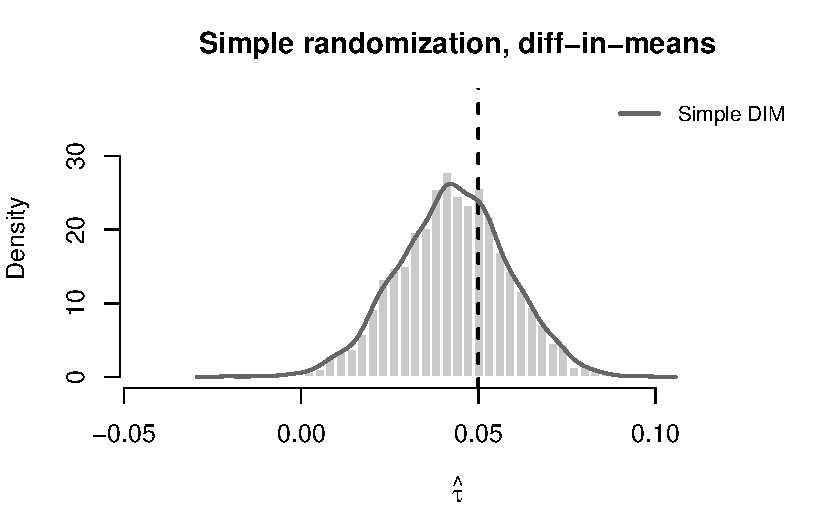
\includegraphics[width=0.72\textwidth]{figures/sim_simple.pdf}
\end{center}
\footnotesize
\textbf{Actual SD} of $\hat\tau$ across reps: 0.016.
\textbf{Mean HC2 SE} from a single \texttt{lm}: 0.016.
The estimator is wide, but the SE accurately knows it.
\end{frame}


% =====================================================================
\section{Covariate Adjustment}
% =====================================================================

\begin{frame}{Covariate adjustment: motivation}
\small
\begin{itemize}
\item<1-> A pre-treatment $X$ that predicts $Y$ also predicts $\hat\tau$'s
  noise: when $T$ and $C$ groups happen to differ on $X$, $\hat\tau$ moves.
\item<2-> ``Adjusting'' for $X$ removes that contribution to the variance
  of $\hat\tau$. \medskip
\item<3-> Crucially: we are \textit{not} adjusting to remove bias.
  Randomization already handled bias. We are adjusting to \textbf{reduce
  variance}.
\item<4-> Rule of thumb: \textit{covariate adjustment helps to the extent
  $X$ predicts $Y$, not to the extent $X$ ``is a variable you have.''}
\item<5-> Strong predictors (\texttt{past\_turnout}) help a lot. Weak
  predictors (\texttt{partisan strength}) barely help. There's no harm
  in including both, in moderation.
\end{itemize}
\end{frame}


\begin{frame}{Adjustment ``perfects'' the balance the regression sees}
\small
\begin{itemize}
\item<1-> Why does OLS with $X$ work? Loosely: it splits $D$ into the part
  predicted by $X$ and the part orthogonal to $X$, and uses only the
  orthogonal part to estimate $\tau$. \medskip
\item<2-> By construction, the ``effective'' treatment indicator the
  regression uses is \textit{exactly balanced} on $X$. The chance
  imbalance from the previous slide is gone. \medskip
\item<3-> So whatever variance was being driven by that imbalance also
  goes away. \medskip
\item<4-> (Formal version --- the Frisch-Waugh-Lovell theorem --- in the
  appendix.)
\end{itemize}
\end{frame}


\begin{frame}{The Lin estimator (one slide)}
\small
The simplest covariate-adjusted estimator is just:
\[
Y_i = \alpha + \tau D_i + \be' X_i + \epsilon_i \qquad
\text{(plain OLS, fine in large samples)}
\]

\medskip
Lin (2013) showed a small modification is essentially always weakly better:
\[
Y_i = \alpha + \tau_{Lin} D_i + \be_1' (X_i - \bar X) +
\be_2' \, D_i \cdot (X_i - \bar X) + \epsilon_i
\]
\begin{itemize}
\footnotesize
\item Demean $X$, then interact with $D$.
\item $\tau_{Lin}$ is interpretable directly as an ATE.
\item Removes a small ($O(1/N)$) bias from plain regression adjustment that
  Freedman (2008) flagged.
\item Treat this as your default. Pre-specify the covariates.
\end{itemize}
\medskip
\onslide<2->
(Detailed derivation, why demeaning matters, Freedman vs.\ Lin discussion:
appendix.)
\end{frame}


\begin{frame}{Simulation: + Lin-adjusted}
\begin{center}
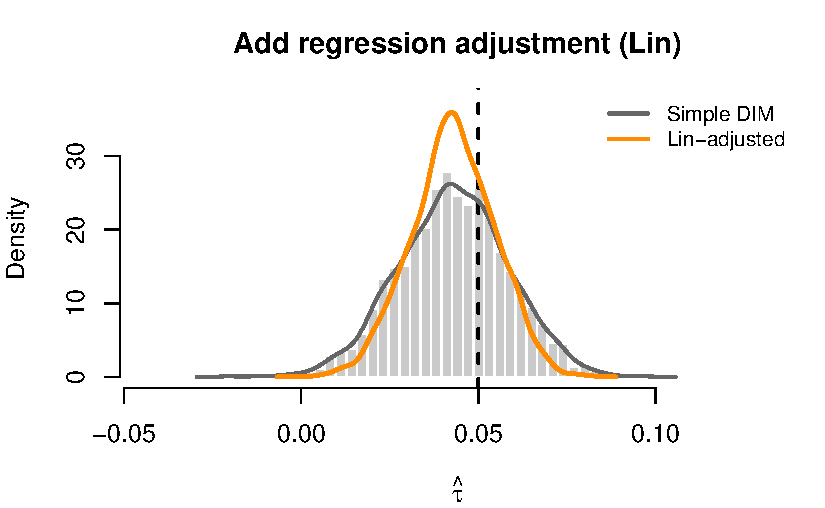
\includegraphics[width=0.72\textwidth]{figures/sim_adjusted.pdf}
\end{center}
\footnotesize
Same 2{,}000 experiments. The grey bars are the simple-DIM baseline. The
orange curve is the Lin-adjusted estimator. Same center, $\sim$25\%
tighter. \\[0.4ex]
\textbf{SD(actual)} = 0.012 \quad
\textbf{Mean HC2 SE} = 0.012 \quad ($\Rightarrow$ HC2 still nails it)
\end{frame}


% =====================================================================
\section{Blocking}
% =====================================================================

\begin{frame}{Blocking: build the balance in, don't hope for it}
\small
\begin{itemize}
\item<1-> Adjustment fixes chance imbalances \textit{after} they happen, in
  the analysis.
\item<2-> Blocking prevents them \textit{before} they happen, in the
  design:
  \begin{itemize}
  \footnotesize
  \item Pre-stratify on a strong predictor (e.g., quartiles of
    \texttt{past\_turnout}).
  \item Randomize within each stratum (block).
  \end{itemize}
\item<3-> The randomization is still doing its job --- it's still
  balancing all the unobserved stuff in expectation. We're just not
  asking it to do the work on the things we already measured. \medskip
\item<4-> \textbf{Slogan:} block what you can, adjust for what you can't.
\end{itemize}
\end{frame}


\begin{frame}{Blocking: the estimator}
\small
\onslide<1-> Within each block $j$, compute the block-specific
diff-in-means $\hat\tau_j$. Then weight by block size:
\[
\hat\tau_B = \sum_{j=1}^J \frac{N_j}{N}\, \hat\tau_j
\]

\medskip
\onslide<2-> Equivalently, when treatment probability is the same in every
block, we can run OLS with block fixed effects:
\[
Y_i = \alpha + \tau D_i + \sum_{j=2}^J \beta_j B_{j[i]} + \epsilon_i
\]
\onslide<3->
\begin{itemize}
\footnotesize
\item Caveat: with unequal treatment probabilities across blocks, plain
  block-FE OLS gives a (weighted) ATE that may not be what you want; use
  the block-weighted form above. (Aside on ``weird weighting'' later in
  the course.)
\end{itemize}
\end{frame}


\begin{frame}{Simulation: + blocked}
\begin{center}
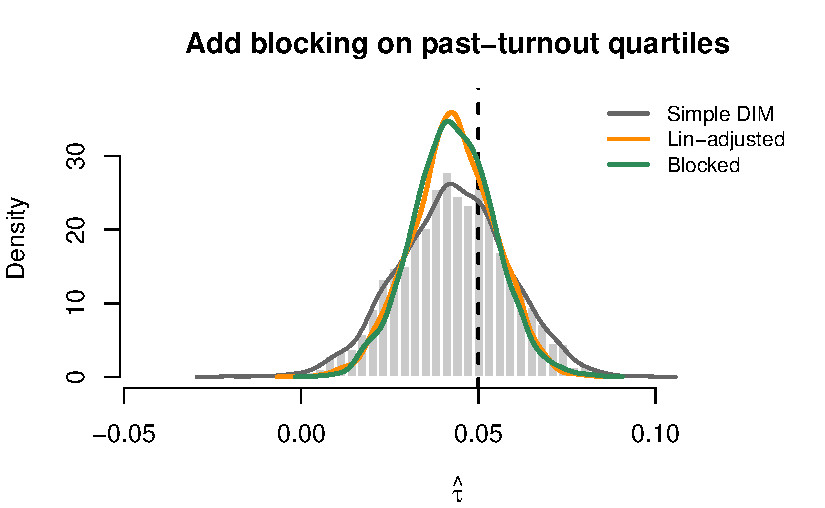
\includegraphics[width=0.72\textwidth]{figures/sim_blocked.pdf}
\end{center}
\footnotesize
Add the green curve: blocking on \texttt{past\_turnout} quartiles. Lands
essentially on top of the Lin-adjusted curve in this DGP. \\[0.4ex]
\textbf{SD(actual)} = 0.012 \quad \textbf{Mean HC2 SE} = 0.012 \quad
(also fine) \\
Sometimes blocking strictly beats post-hoc adjustment; in well-behaved
cases the two converge.
\end{frame}


\begin{frame}{When does blocking help most? Intuition}
\begin{itemize}
\item Blocking helps a lot when the blocking variable \textit{strongly
  predicts $Y$}. Then within-block variation in $Y$ is small, so the
  diff-in-means within each block is sharp.
\item Blocking on something unrelated to $Y$ is essentially free, but
  also essentially useless.
\item In our sim, we blocked on \texttt{past\_turnout}, which is the
  dominant predictor of voting --- so we got a large gain.
\item (Formal variance comparison in the appendix.)
\end{itemize}
\end{frame}


\begin{frame}{A canonical real example: Gerber, Green, \& Larimer (2008)}
\small
\begin{itemize}
\item Field experiment on social pressure and voter turnout (Michigan
  primary, 2006).
\item Several mailings, including one revealing each voter's past turnout
  to their neighbors.
\item \textbf{Design:}
  \begin{itemize}
  \footnotesize
  \item Blocked on household composition and prior vote history.
  \item Randomized at the \textit{household} level, not the individual
    level. (Foreshadows the next section.)
  \end{itemize}
\item \textbf{Result:} the ``neighbors'' treatment moved turnout by
  ${\approx}\,8$ percentage points --- enormous for a piece of mail.
\item \textbf{Why we cite this design:} the blocking + household clustering
  match the situation we're simulating today. Their estimator is precise
  because the design earned it, not because the analysis fixed it.
\end{itemize}
\end{frame}


% =====================================================================
\section{Non-Independence and Clustering}
% =====================================================================

\begin{frame}{Two problems from non-independence}
\small
So far we've assumed observations are (conditionally) independent. Real
settings often violate this --- voters in the same precinct, students in
the same classroom, repeated measures on the same person. \medskip

Two distinct things can go wrong, and they need different fixes:
\begin{enumerate}
\item \textbf{Clustered assignment.} Treatment is assigned at the group
  level (precinct, village, school). The point estimate itself becomes
  noisier --- the experiment is worse.
\item \textbf{Dependent residuals.} Even with individual assignment,
  residuals can be correlated within a group, and SEs that ignore this
  can be wrong.
\end{enumerate}
\end{frame}


\begin{frame}{Simulation: cluster-randomize at the precinct level}
\begin{center}
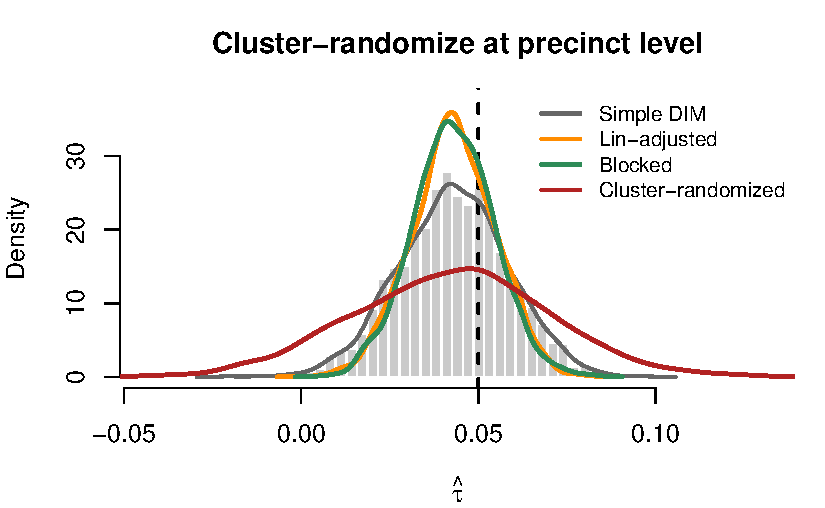
\includegraphics[width=0.72\textwidth]{figures/sim_clustered.pdf}
\end{center}
\footnotesize
Same DGP, same $\tau$, but treatment is now assigned at the
\textbf{precinct} level (everyone in a precinct gets the same $D$). The
red curve is enormously wider than the individual-assignment baseline.
Each precinct contributes essentially one ``decision'' --- with 100
precincts, that's a much smaller experiment than $N = 4{,}000$ suggests.
\end{frame}


\begin{frame}{HC2 is wrong here. CR-SE fixes it.}
\small
\begin{center}
\begin{tabular}{lccc}
\toprule
Estimator & SD(actual) & HC2 SE & CR-SE (precinct) \\
\midrule
Simple DIM (\texttt{lm(Y\~{}D)})       & 0.016 & \textbf{0.016} & 0.016 \\
Lin-adjusted                            & 0.012 & \textbf{0.012} & --- \\
Blocked (block FEs)                     & 0.012 & \textbf{0.012} & --- \\
Cluster-randomized                      & \textbf{0.028} & 0.016 & \textbf{0.028} \\
\bottomrule
\end{tabular}
\end{center}
\onslide<2->
\begin{itemize}
\item HC2 assumes independent observations. With cluster-level assignment
  everyone in a precinct shares the same $D$ --- that assumption is
  badly violated.
\item Cluster-robust SE (clustered at the precinct level) recovers the
  actual sampling variance almost exactly. In R:\\
  \texttt{\quad sandwich::vcovCL(fit, cluster = precinct\_id)}.
\item The CR-SE is not magic --- it estimates the actual within-cluster
  residual covariance from the data, not the worst-case ``$N = $ number
  of clusters.''
\end{itemize}
\end{frame}


\begin{frame}{When do you actually need CR-SEs? The principle}
\small
\textbf{You need cluster-robust SEs when there is a source of common
influence on outcomes within a cluster, \textit{and} that influence is
not canceled out by treatment variation within the cluster.}
\medskip
\onslide<2->
Two ingredients are required:
\begin{enumerate}
\item A cluster-shared component in $Y$ (a precinct effect $u_c$, a
  school's teacher quality, a household's news diet, a person's baseline
  level in panel data).
\item A failure of within-cluster $T/C$ variation to cancel that
  component out of the residuals.
\end{enumerate}
\medskip
\onslide<3->
Either ingredient \textit{alone} is harmless:
\begin{itemize}
\footnotesize
\item No cluster-shared component $\Rightarrow$ residuals are iid
  $\Rightarrow$ HC2 is fine. (Even cluster-randomized assignment has no
  penalty --- we verified this in simulation.)
\item Cluster-shared component, but balanced individual assignment within
  cluster $\Rightarrow$ the diff-in-means cancels $u_c$ $\Rightarrow$
  HC2 is fine.
\end{itemize}
\medskip
\onslide<4->
\textbf{Both at once is the dangerous case.} Cluster-shared $u_c$
\textit{and} no within-cluster treatment variation to break it up. That
is exactly our cluster-randomized precinct example.
\end{frame}


\begin{frame}{Where ``both at once'' shows up in practice}
\small
\begin{itemize}
\item<1-> \textbf{Cluster-randomized treatment} (precincts, villages,
  schools, clinics). Same $D$ for the whole cluster; $u_c$ rides with $D$.
\item<2-> \textbf{Repeated measures / panel data with unit-level
  treatment.} Same person observed many times, ``treated'' or ``control''
  the whole way through. The person plays the role of the cluster; their
  idiosyncratic level rides with $D$. Mechanically identical to
  cluster-randomized.
\item<3-> \textbf{Spillovers within a group.} Treating one household
  member effectively treats the rest, so the whole household shares one
  effective $D$.
\item<4-> \textbf{Treatment probabilities that differ by cluster.} Even
  with individual assignment, asymmetric $T/C$ proportions stop $u_c$
  from cancelling cleanly.
\item<5-> \textbf{Heterogeneous treatment effects by cluster.} $\tau_c$
  varies across clusters; the residual carries a $\tau_c D_i$ piece that
  is cluster-correlated on the treated side and doesn't cancel.
\end{itemize}
\medskip
\onslide<6->
\textbf{Subtle but real:} ``students within schools'' with individual,
balanced random assignment within school is \textit{not} automatically a
case for CR-SEs. It usually is in practice --- because one of (1)--(5) is
hiding in the design --- but not from the nesting alone.
\end{frame}


\begin{frame}{Catches with CR-SEs}
\small
\begin{itemize}
\item<1-> \textbf{They are not free.} CR-SEs can be substantially
  conservative when within-cluster residual correlation is weak ---
  intervals widen, power drops, with no coverage gain.
\item<2-> \textbf{Few clusters is a real problem.} The standard CR-SE
  estimator (\texttt{vcovCL} / Liang--Zeger) is downward biased with
  $C \lesssim 30$--$50$ clusters; rejection rates from the resulting
  $t$-tests can be far above nominal.
\item<3-> \textbf{Fixes for few clusters:}
  \begin{itemize}
  \footnotesize
  \item Wild cluster bootstrap (Cameron, Gelbach \& Miller 2008):
    \texttt{fwildclusterboot} in R, \texttt{boottest} in Stata.
  \item Randomization inference at the cluster level.
  \item Aggregate to the cluster level and run the analysis there.
  \end{itemize}
\end{itemize}
\end{frame}


% =====================================================================
\section{Wrap}
% =====================================================================

\begin{frame}{Same experiment, four designs and analyses}
\begin{center}
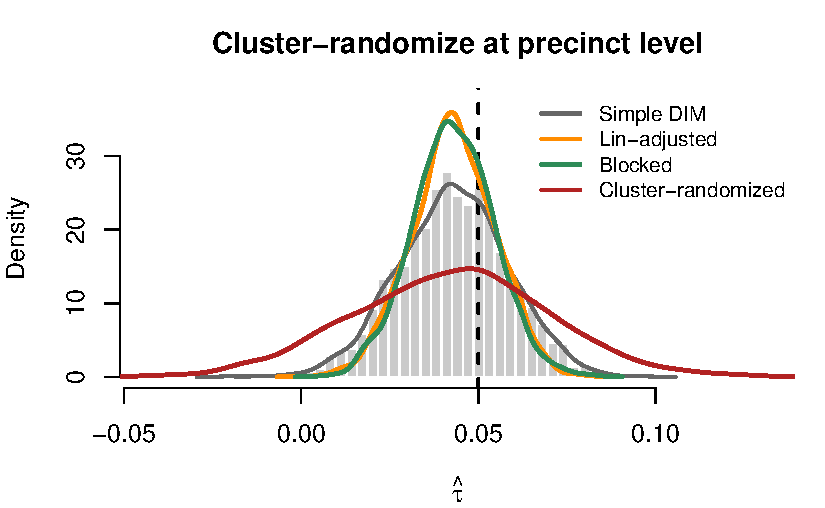
\includegraphics[width=0.78\textwidth]{figures/sim_combined.pdf}
\end{center}
\small
Same DGP, same true $\tau = 0.05$. None of these estimators is biased ---
they differ entirely in precision. Both \textit{design} (blocking,
avoiding unnecessary clustering) and \textit{analysis} (covariate
adjustment) deliver real gains.
\end{frame}


\begin{frame}{Takeaways}
\begin{itemize}
\item \textbf{Unbiasedness is not enough.} The same experiment can be run
  more or less precisely; that's what we're paying attention to today.
\medskip
\item \textbf{Adjustment works.} Covariate adjustment recovers real
  precision when $X$ predicts $Y$. Use Lin's interacted form, with HC2
  SEs, and pre-specify the covariates.
\medskip
\item \textbf{Design works too, often without paying anything for it.}
  Block on what you can; adjust for what you can't. The two are
  complements, not substitutes.
\medskip
\item \textbf{Cluster on the source of dependence in your residuals},
  not on every group you can think of. Watch the few-clusters case and
  reach for the wild bootstrap when needed.
\medskip
\item Next: what if we can't randomize at all?
  \textbf{Selection on observables.}
\end{itemize}
\end{frame}


% =====================================================================
\appendix
% =====================================================================

\begin{frame}
\begin{center}
\Large Appendix
\end{center}
\end{frame}


\begin{frame}{Frisch-Waugh-Lovell (FWL) theorem}
\small
Two facts:
\begin{enumerate}
\footnotesize
\item Any bivariate regression of $Y$ on $X$ has
  $\hat\beta = \widehat\Cov(Y,X) / \widehat\Var(X)$.
\item The coefficient on the $k$th regressor in a multivariate regression
  can be obtained by (i) regressing $X_k$ on the other $X$'s and saving the
  residual $\tilde X_k$, then (ii) regressing $Y$ (or its residual
  $\tilde Y$) on $\tilde X_k$.
\end{enumerate}
\medskip
Together:
\[
\hat\beta_k =
\frac{\widehat\Cov(\tilde Y_i, \tilde X_{ki})}{\widehat\Var(\tilde X_{ki})}
\]
\end{frame}


\begin{frame}{Why experimental findings are robust to specification}
\small
Apply FWL to $D$:
\[
\hat\beta_D =
\frac{\widehat\Cov(\tilde Y_i, \tilde D_i)}{\widehat\Var(\tilde D_i)}
\]
where $\tilde D_i$ is the residual from regressing $D_i$ on $X_i$.
\medskip
\begin{itemize}
\footnotesize
\item Under randomization, $D \indep X$, so on average
  $\tilde D \approx D$.
\item Hence adjusting for $X$ doesn't move $\hat\beta_D$ much in expectation
  --- it just removes the variance contribution from chance imbalances.
\item This is why experimental results are typically robust to
  ``what did you control for?''
\end{itemize}
\end{frame}


\begin{frame}{Lin (2013): why the demeaning?}
\small
\[
Y_i = \alpha + \tau_{Lin} D_i + \be_1' (X_i - \bar X) +
\be_2' \, D_i (X_i - \bar X) + \epsilon_i
\]
\begin{itemize}
\footnotesize
\item $\E[Y_i \mid D_i = 0, X_i = \bar X] = \alpha$
\item $\E[Y_i \mid D_i = 1, X_i = \bar X] = \alpha + \tau_{Lin}$
\item So $\tau_{Lin}$ is the comparison of treated vs.\ control
  \textit{at the mean of $X$}.
\item Because $\E_X[\text{ATE}(X)] = \tau_{Lin}$ for this model, it
  recovers the ATE without assuming constant treatment effects.
\item Plain OLS without the interaction works in large samples but is
  biased $O(1/N)$ (Freedman 2008). Lin's form removes this and is now
  standard practice.
\end{itemize}
\end{frame}


\begin{frame}{When does blocking help? (variance comparison)}
\small Models for complete and block-randomized designs:
\begin{small}
\begin{eqnarray*}
Y_i &=& \alpha + \tau_{CR} D_i + \textcolor{red}{\varepsilon_i} \\
Y_i &=& \alpha + \tau_{BR} D_i + \sum_{j=2}^J \beta_j B_{j[i]} +
        \textcolor{blue}{\varepsilon^{*}_i}
\end{eqnarray*}
\end{small}
Then
\begin{small}
\begin{eqnarray*}
\Var[\hat\tau_{CR}] &=&
  \frac{\textcolor{red}{\sigma^2_\varepsilon}}
       {\sum_i (D_i - \bar D)^2} \\
\Var[\hat\tau_{BR}] &=&
  \frac{\textcolor{blue}{\sigma^2_{\varepsilon^*}}}
       {\sum_i (D_i - \bar D)^2 (1 - R_D^2)}
\end{eqnarray*}
\end{small}
where $R_D^2$ is from regressing $D$ on the block dummies.
\end{frame}


\begin{frame}{When does blocking help? (intuition)}
\small
\begin{itemize}
\item If treatment proportions are the same in every block, $R_D^2 = 0$
  and the denominator is unchanged --- blocking doesn't \textit{cost} you
  anything.
\item If the blocks strongly explain $Y$, then
  $\textcolor{blue}{\sigma^2_{\varepsilon^*}} \ll
   \textcolor{red}{\sigma^2_\varepsilon}$ --- blocking \textit{wins} a lot.
\item Combine: blocking on a strong predictor of $Y$, with equal-share
  randomization, weakly improves precision and usually does so a lot.
\end{itemize}
\end{frame}


\begin{frame}{Cluster-robust variance: a sketch}
\small
For OLS $\hat\beta = (X'X)^{-1} X'Y$, the cluster-robust variance is
\[
\widehat\Var_{CR}(\hat\beta) =
(X'X)^{-1}
\Bigg(\sum_{c=1}^C X_c' \hat e_c \hat e_c' X_c \Bigg)
(X'X)^{-1}
\]
\begin{itemize}
\footnotesize
\item $X_c$ and $\hat e_c$ are the design matrix and residuals for cluster
  $c$.
\item This collapses cluster-level scores, so it allows arbitrary
  intra-cluster correlation in residuals while assuming clusters are
  independent.
\item The ``effective $N$ = $C$'' approximation is the limit case
  $\rho \to 1$. The actual penalty is data-driven via $\hat e_c$.
\item With $C \lesssim 30$, this estimator is downward biased; use a wild
  cluster bootstrap (Cameron, Gelbach, \& Miller 2008) instead.
\end{itemize}
\end{frame}


\begin{frame}{LPM caveats (binary outcomes)}
\small
Using OLS / LPM with a binary $Y$:
\begin{itemize}
\footnotesize
\item \textbf{Pro:} unbiased for the ATE under random assignment;
  coefficients are interpretable as probability differences; works in
  every standard software environment.
\item \textbf{Cons:}
  \begin{itemize}
  \item Predicted probabilities can fall outside $[0,1]$.
  \item Heteroskedasticity is built in --- use robust SEs.
  \item In observational settings with extreme covariates, linearity can
    be a poor approximation.
  \end{itemize}
\item For the experimental settings in this lecture, none of these are
  reasons to abandon LPM.
\end{itemize}
\end{frame}


\end{document}
